\section{In-context learning}

A surprising property of large language models is their emergent ability to learn \textit{in-context}, that is, their ability to learn a task without updating any parameters at all. The name `in-context' comes from the fact that the learning is done by simply including several examples or a task description (or both!) prepended to a test input present to the model

For example, for a question-answering task, to make a 2-shot prediction for a test input `Why is the sky blue?', rather than presenting the input:

\texttt{Why is the sky blue?\textless generate\textgreater}

we would simply prepend our 2 examples to the input:

\texttt{Who is the US president? Joe Biden What is earth's tallest mountain? Mount... \\
Everest Why is the sky blue?\textless generate\textgreater}

In addition to few-shot in-context learning, models can often improve their zero-shot generalization if the input is formatted in a particular manner; for example, adding a \texttt{Q:} and \texttt{A:} prefix to the input and label, respectively:

\texttt{Q: Why is the sky blue? A:\textless generate\textgreater}

Finally, these two approaches can be combined, for example adding the \texttt{Q:} and \texttt{A:} markers to each example in the context as well as the test input.

\begin{enumerate}[label={2.\alph*}]
    \item \points{3a} {\bf Implement Parameter-efficient Fine Tine}

Finish the implementation for each version of parameter-efficient fine-tuning for GPT-2-Medium in 

\texttt{ft.py:parameters\_to\_fine\_tune()}:

\begin{enumerate}[label=(\roman*)]
    \item \texttt{last}: Fine-tune only the last 2 transformer blocks
    \item \texttt{first}: Fine-tune only first 2 transformer blocks
    \item \texttt{middle}: Fine-tune only middle 2 transformer blocks
\end{enumerate}
This step simply requires selecting the correct subset of parameters for each version listed above in 

\texttt{parameters\_to\_fine\_tune()}. Keep in mind you should be returning an iterable of \texttt{nn.Parameter} here, not \texttt{nn.Module}.
    \item {\bf Evaluate on bAbI}

\begin{enumerate}[label=(\roman*)]
    \item \points{2bi} {\bf Run ICL on bAbI}

First, evaluate $k$-shot in-context performance on bAbI for GPT-2-medium (355M parameters) and full-size GPT-2 (1.5B parameters) for various values of $k$ with the command:
    
\texttt{\small python3 main.py --task run\_icl --model med,full --dataset babi --k 0,1,16}

Plot the results with the command:

\texttt{\small python3 main.py --task plot\_icl --model med,full --dataset babi --k 0,1,16}

Your plots should look like:
\begin{figure}[H]
    \centering
    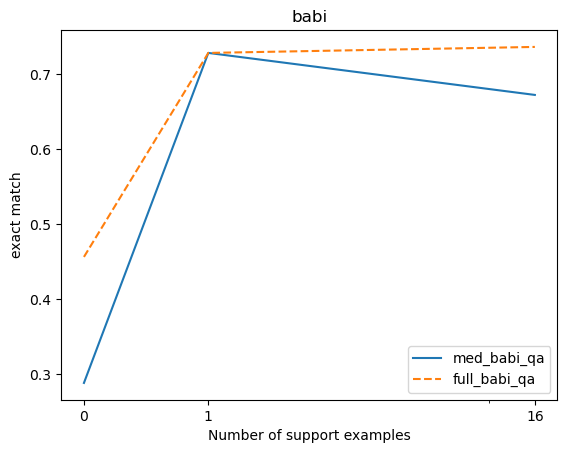
\includegraphics[width=0.75\linewidth]{./figures/q2_babi_plot}
    \caption{\textit{k}-shot in-context performance on bAbI for GPT-2-medium and full-size GPT-2 for various values of \textit{k}}
\end{figure}

    \item \points{2bii} {\bf Reason on ICL on bAbI}


What relationship(s) do you notice between model scale and few-shot performance?
\end{enumerate}

    \item {\bf Evaluate on XSum}

\begin{enumerate}[label=(\roman*)]
    \item \points{2ci} {\bf Run ICL on XSum}

Now let's evaluate several different prompt formats on the XSum dataset. With and without a task description in the prompt, evaluate zero-shot and few-shot performance for XSum on GPT-2-Medium with the command:

\texttt{\small python3 main.py --task run\_icl --model med,full --dataset xsum --k 0,1,4 \textbackslash \\
\phantom{asdf}--prompt none,tldr,custom}

Note that we use much smaller $k$ than in the previous problem, because we must fit all $k$ examples into the model's context window, which is only 1024 tokens. The fixed context window length is one limitation of in-context learning.

\textbf{The $k=4$ XSum evaluation on full-size GPT-2 may take approximately 40 minutes on your Azure instance for each prompt mode}; this is expected, and is another downside of in-context learning (we need to process a much longer input, containing the prompt, compared to a fine-tuned model that just processes the test input).

Plot the zero-shot and few-shot performance of GPT-2 on XSum:

\texttt{\small python3 main.py --task plot\_icl --model med,full --dataset xsum --k 0,1,4 \textbackslash \\
\phantom{asdf}--prompt none,tldr,custom}

Your plot should look like:
\begin{figure}[H]
    \centering
    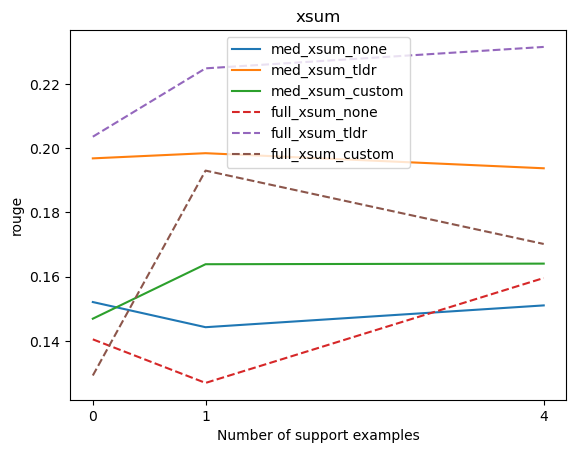
\includegraphics[width=0.75\linewidth]{./figures/q2_xsum_plot}
    \caption{\textit{k}-shot in-context performance of GPT-2-medium and full-size GPT-2 for various values of \textit{k} on XSum}
\end{figure}


    \item \points{2cii} {\bf Reason on ICL on XSum}

How does the performance of the \texttt{TL;DR:} prompt compare with no prompt formatting? What was your custom prompt format, and how did it compare with \texttt{TL;DR:}? Discuss the relative performance of the different prompts in the zero-shot, one-shot, and few-shot settings.

\end{enumerate}

\end{enumerate}